\documentclass[12pt,a4paper]{article}
\usepackage[utf8]{inputenc} %polskie znaki
\usepackage[T1]{fontenc}	%polskie znaki
\usepackage{amsmath}		%matematyczne znaczki :3
\usepackage{enumerate}		%Dodatkowe opcje do funkcji enumerate
\usepackage{geometry} 		%Ustawianie marginesow
\usepackage{graphicx}		%Grafika
\usepackage{wrapfig}		%Grafika obok textu
\usepackage{float}			%Allows H in fugire
%\pagestyle{empty} 			%usuwa nr strony

\newgeometry{tmargin=2cm, bmargin=2cm, lmargin=2cm, rmargin=2cm} 

\begin{document}
	\begin{center}
		\LARGE Trygonometria cz. 2
	\end{center}
	\vspace{1cm}
	
	
	\begin{enumerate}[1.]	
		\item Dla podanej funkcji trygonometrycznej i kąta wyznacz jej pozostałe funkcje trygonometryczne:
		
		
		\begin{enumerate}[a)] \begin{tabular}{p{7cm} p{7cm}} \item 		
				$\sin\alpha=\frac{5}{13} \qquad \alpha\in(90^\circ,180^\circ)$& \vspace{0.4cm} 	\item $\cos\alpha=0,5\qquad\alpha\in(90^\circ,180^\circ)$ \\
				\item $\cos\alpha=\frac{\sqrt{5}}{5}\qquad\alpha\in(90^\circ,180^\circ)$ &\item $\text{ctg } \alpha=\frac{1}{\sqrt{3}}\qquad\alpha\in(90^\circ,180^\circ)$ \\
				\item $\text{tg }\alpha=2\qquad\alpha\in(90^\circ,180^\circ)$ &\item $\sin\alpha=\frac{1}{\sqrt{3}}\qquad\alpha\in(90^\circ,180^\circ)$ \\
		\end{tabular} \end{enumerate}
		
		\item Oblicz korzystając ze wzorów redukcyjnych
		\begin{enumerate}[a)] \begin{tabular}{p{4cm} p{4cm} p{4cm}}
				\item $\sin 120^\circ=$& \vspace{0.25cm}\item$\cos 120^\circ=$& \vspace{0.25cm} \item$\sin 150^\circ=$\\
				\item$\text{tg } 150^\circ$=&\item$\sin 225^\circ$ =&\item$\cos 420^\circ$=\\
				\item$\cos 330^\circ$=&\item$\sin (-210^\circ)$=&\item$\text{tg }210^\circ$=\\
				\item$\sin1050^\circ$=&\item$\cos(-600^\circ)$=&\item$\text{ctg }(-450^\circ)$=\\
		\end{tabular} \end{enumerate}
	
		\item Oblicz 
		\begin{enumerate}[a)] \begin{tabular}{p{4cm} p{4cm} p{4cm}}
				\item $\sin 75^\circ=$& \vspace{0.25cm}\item$\cos 15^\circ=$& \vspace{0.25cm} \item$\text{tg } 105^\circ=$\\
		\end{tabular} \end{enumerate}
	
	\item Rozwiąż trójkąty: (oblicz wszystkie boki, kąty oraz jego pole)
	
	\begin{figure}[h]
		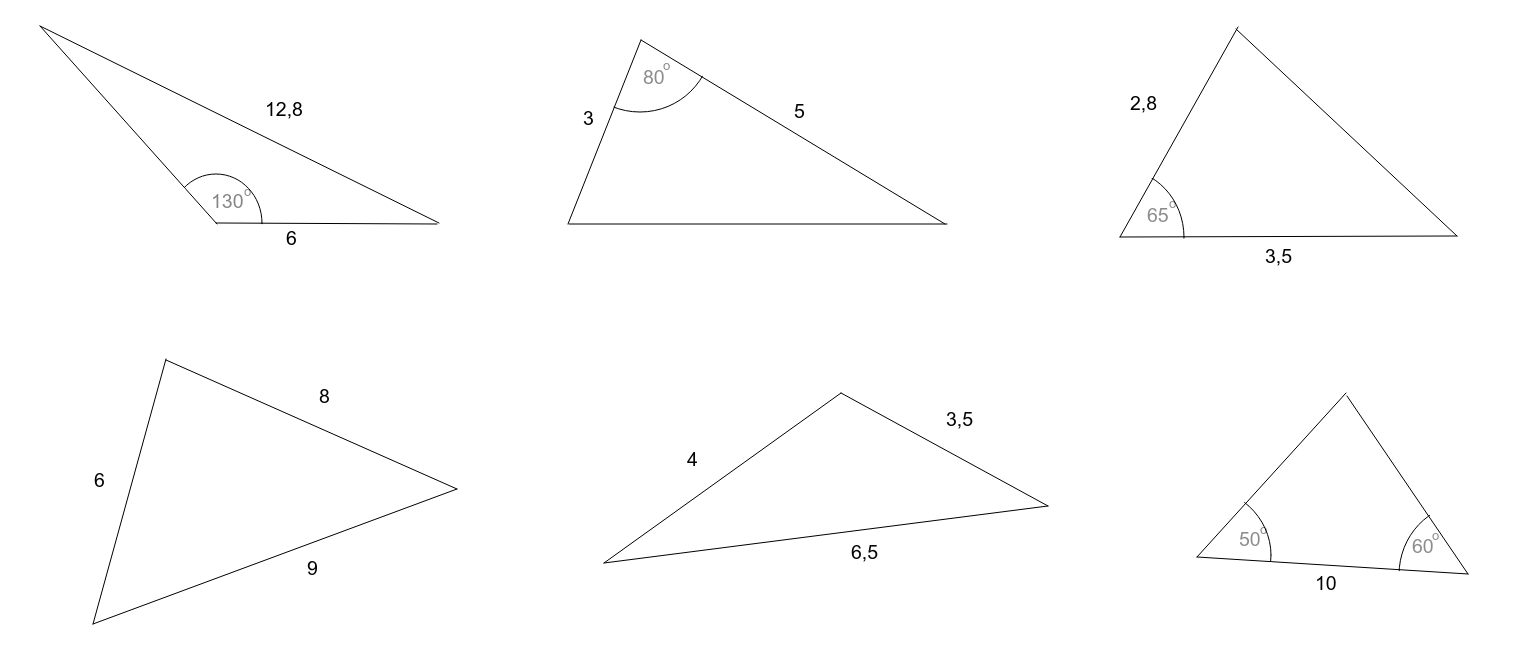
\includegraphics[scale=0.31]{t2_1}
	\end{figure}

	\newpage
	\item Dany jest trójkąt $ABC$ o bokach 4 i 6 oraz kącie między nimi równy $60^\circ$. Oblicz pole tego trójkąta.
	\item Dany jest trójkąt $ABC$ o bokach $|AB|=8$, $|BC|=12$ i $|AC|=7$. Oblicz największy kąt tego trójkąta.
	\item W trójkącie $ABC$ mamy dane $|BC|=4$ i $\angle BAC=150^\circ$. Oblicz promień koła opisanego na tym trójkącie.
	\item W trójkącie $ABC$ są dane $|BC|=5$, $\angle BAD=48^\circ$ oraz $\angle ACB=70^\circ$. Oblicz długość boku $AC$ tego trójkąta.
	\item Dany jest trójkąt $ABC$, którego boki są równe $|AB|=4,5$, $|BC|=6,2$ i $|AC|=3,7$. Oblicz najmniejszy kąt tego trójkąta.
	\item Oblicz pole trójkąta równoramiennego o ramieniu równym 8 i kącie przy podstawie $75^\circ$.
	\item W trójkącie $ABC$ dane są boki $|AB|=\sqrt{14}$, $|BC|=3\sqrt{2}$ i $|AC|=\sqrt{2}$. Oblicz kąt przy wierzchołku $C$.
	\item W trójkącie $ABC$ wiemy, że $|AC|=4$, $|AB|=|BC|+2$ oraz $\angle ACB = 60^\circ$. Oblicz kąty $\angle BAC$ i $\angle ABC$.

		
	\end{enumerate}
\end{document}